The 'sndfile' plugin reads sound files and adds their content to the audio signal. Playback can be controlled by the session timeline, triggered by OSC messages, or independent of both. The libsndfile library (\url{http://www.mega-nerd.com/libsndfile/}) is used internally, so all file and sample formats supported by this library are also supported by this plugin.

\definecolor{shadecolor}{RGB}{255,230,204}\begin{snugshade}
{\footnotesize
\label{attrtab:sndfile}
Attributes of element {\bf sndfile}\nopagebreak

\begin{tabularx}{\textwidth}{lXl}
\hline
name & description (type, unit) & def.\\
\hline
\hline
\indattr{attribution} & attribution of license, if applicable (string) & \\
\hline
\indattr{channel} & First sound file channel to be used, zero-base (uint32) & 0\\
\hline
\indattr{channelorder} & Channel order in case of First Order Ambisonics files, ``FuMa'', ``ACN'' or ``none'' (string, FuMa|ACN|none) & \\
\hline
\indattr{length} & length of sound sample, or 0 to use whole file length (double, s) & 0\\
\hline
\indattr{level} & level, meaning depends on \attr{levelmode} (double, dB) & -inf\\
\hline
\indattr{levelmode} & level mode, ``rms'', ``peak'' or ``calib'' (string) & rms\\
\hline
\indattr{license} & license type (string) & \\
\hline
\indattr{loop} & loop count or 0 for infinite looping (uint32) & 1\\
\hline
\indattr{loopcrossexp} & exponent of von-Hann crossfade for seamless loop (float) & 1\\
\hline
\indattr{loopcrosslen} & duration of crossfade for seamless loop (float, s) & 0\\
\hline
\indattr{mute} & Load muted (bool) & false\\
\hline
\indattr{name} & Sound file name (string) & \\
\hline
\indattr{normalization} & Normalization in case of First Order Ambisonics files. (string, FuMa|SN3D) & FuMa\\
\hline
\indattr{position} & Start position within the scene (double, s) & 0\\
\hline
\indattr{rampend} & von-Hann ramp duration at end of sound (float, s) & 0\\
\hline
\indattr{rampstart} & von-Hann ramp duration at start of sound (float, s) & 0\\
\hline
\indattr{resample} & Allow resampling to current session sample rate (bool) & false\\
\hline
\indattr{start} & Start position within the file (double, s) & 0\\
\hline
\indattr{transport} & Use session time base (bool) & true\\
\hline
\indattr{triggered} & Use OSC variable `/loop' to trigger playback (ignores attributes `position' and `loop') (bool) & false\\
\hline
\indattr{weighting} & level weighting for RMS mode (f-weight) & Z\\
\hline
\end{tabularx}
}
\end{snugshade}


\paragraph{Multi-channel sound files}
%
If the plugin receives multiple channels (e.g., when used in a receiver, a diffuse sound field or a multichannel route), all channels starting with the channel number \attr{channel} are returned. If the file does not contain a sufficient number of channels, silence is returned for all channels not available in the sound file.

If the number of plugin channels (not sound file channels) is four, and the attribute \attr{channelorder} is not ``none'', a First Order Ambisonics sound file with SN3D normalization is assumed. In that case, the \attr{channelorder} should be set to the correct channel order.

\paragraph{Calibration of levels}
%
In the level mode ``rms'', the RMS value of the first used channel
will be used for adjusting the level, i.e., all channels will be
scaled with the same value such that the first channel has the
RMS level \attr{level}.
\begin{itemize}
\item Level mode ``rms'' scales the signal so the RMS of the first channel corresponds to \attr{level}.

\item Level mode ``peak'' scales the signal so the peak over all channels corresponds to \attr{level}.

\item Level mode ``calib'' scales the signal by \attr{level} minus 93.979~dB.
\end{itemize}
Internally, the signal is measured in Pascal. Therefore, a signal with an RMS value of 1 corresponds to a sound pressure level of 93.979~dB.

Please note that currently the calibration level and the gain of input ports also affects the calibration of the plugins. This is going to change in the future.

\paragraph{Temporal alignment}
%
All times are defined relative to the object time of the sound file plugin's parent object. In most cases this is equivalent to the session time, however, it can be changed with the \attr{start} attribute of the objects in scenes. If the parent object is not within a scene (e.g., a 'route' module), the session time is used.

See also Figure \ref{fig:ap_sndfile} for more details on the time and position conventions.

\begin{figure}[htb]
    \centering
    \fbox{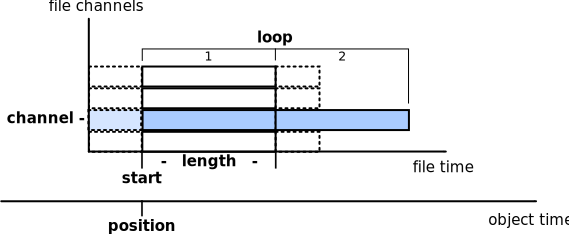
\includegraphics[width=\textwidth]{ap_sndfile}}
    \caption{Temporal alignment of sounds added with the {\tt sndfile} audio plugin.}
    \label{fig:ap_sndfile}
\end{figure}

\paragraph{OSC control}
%
To load a file via OSC, send to the path {\tt /loadfile} (for full
path check the list of OSC variables in TASCAR) with two strings and a
float parameter.
%
The first string is the file name, either as absolute path or relative
to the current session file. The second string is the level mode, see
above for details. The third parameter is the level in dB, again see
above for details.
%
\begin{verbatim}
/scene/in/0/ap0/sndfile/loadfile sound.wav rms 50
\end{verbatim}
%
If an invalid file name or level mode is provided, a warning is
printed to the console running TASCAR (to see such warnings start
TASCAR from a terminal).

List of OSC variables:

\begin{tabularx}{\textwidth}{llX}
\hline
name            & format & description                                                                                             \\
\hline
{\tt /loop}     & i      & In normal mode: Loop count, 0 for infitie loop.                                                         \\
                &        & In ``triggered'' mode: Trigger of playback, number defines number of repetitions, 0 will stop playback. \\
{\tt /position} & f      & Position in scene in seconds                                                                            \\
{\tt /loadfile} & s      & Load file with pre-configured level mode and level                                                      \\
{\tt /loadfile} & ssf    & Load file with level mode and level (see above)                                                         \\
{\tt /mute}     & i      & Mute state                                                                                              \\
\hline
\end{tabularx}

\verb!/position! and \verb!/loop! will affect the file which is loaded next. It will not affect the current file.
